\chapter{Архитектура подсистемы}

\section{Архитектура ПО}

\begin{figure}[H]
    \center{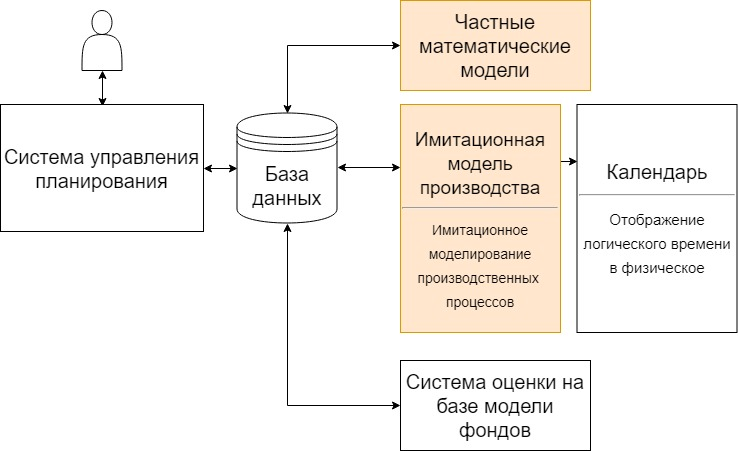
\includegraphics[width=1\linewidth]{fig/arh1.jpg}}
    \caption{Архитектура ПО}
    \label{ris:arh1}
\end{figure}

На рисунке \ref{ris:arh1} представлена архитектуры программного обеспечения. Данная архитектура содержит следующие элементы:

\begin{itemize}
    \item пользовательский интерфейс для взаимодействия с системой, который также позволяет получать информацию о работе системы в виде диаграмм, или графиков; 
    \item система управления планирования взаимодействует со всеми элементами системы и является главным распорядителем задач;
    \item база данных хранит всю информацию о производстве и результаты планирования; 
    \item имитационная модель производства создает план на основе информации из технологической карты и производственного плана;
    \item календарь обрабатывает абсолютные значения, используемые при планировании, и привязывает их к конкретным датам;
    \item частные оптимизационные модели работают с уже сформировавшимся планом, который получен в результате имитационного моделирования. К данному плану применяются алгоритмы оптимизации, зависящие от конкретных целей. Таким целями могут быть: задачи упорядочивания, задачи согласования, задачи распределения, задачи с суммарными критериями оптимизации, задачи с минимаксимальными критериями оптимизации[1, 2].
    \item модель оценки фондов работает с производственными мощностями и дают поверхностную оценку осуществимости заданной цеховой последовательности выпуска;
\end{itemize}

\section{Архитектура имитацонной модели}

Алгоритм планирования состоит из следующих этапов:
\begin{enumerate}
    \item Создание шаблона продуктов на основе заказа. Другими словами воспроизведение порядка операций указанной в технологической карте, статическая система неравенств.
    \item Создание плана на основе заказа. На данном этапе алгоритм создает шаблоны всех продуктов, которые перечислены в заказе, также учитывая количество одноименной продукции.
    \item Пошаговая реализация плана с учетом ресурсных ограничений. Добавление дополнительных ограничений в систему неравенств, которые динамически меняются с каждым шагом планирования.
\end{enumerate}
Работа имитационного моделирования представлена на рисунке \ref{ris:alg}
\begin{figure}[H]
    \center{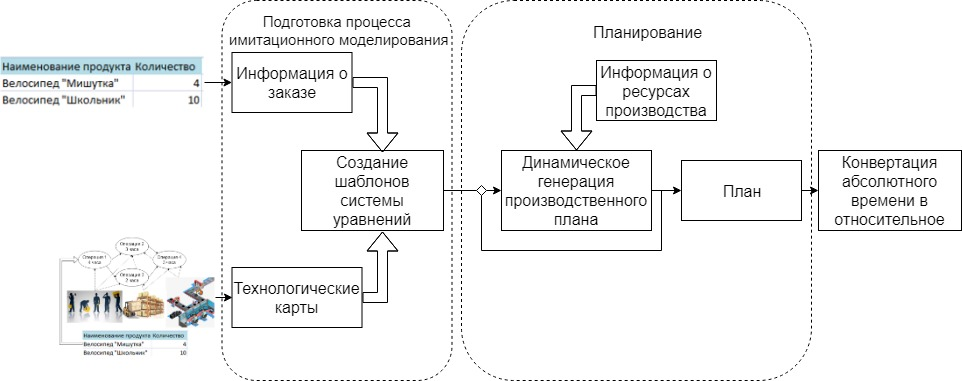
\includegraphics[width=1\linewidth]{fig/alg.jpg}}
    \caption{Визаулизация работы имитацонного моделирования}
    \label{ris:alg}
\end{figure}

\section{Частные оптимизационные модели}

\section{Выбор технологии реализации}

Планированию как вычислительному процессу необходимо большое количество вычислительных ресурсов и их грамотное использование. Это связано с тем фактом, что при планировании перебираются множество возможных вариантов и выбирается только один - лучший (в данном случае имеются в виду алгоритмы оптимального поиска). Когда речь идет о возможности распараллеливания вычислительных ресурсов, требуется технология предоставляющая данную возможность. На данный момент практически все языки программирования имеют функцию распараллеливания, но языки, где это реализовано удобно и без изъянов, немного.  Для построения ядра моделирования был выбран многопоточный, компилируемый язык программирования - golang.

Язык программирпования golang предоставляет следующие возможности:

\begin{enumerate}
    \item Скорость обучения. Часто бывает, что разработчики имеют разный уровень подготовки, поэтому необходим язык который позволяет уменьшить затраты на изучения синтаксиса и как можно быстрее сосредоточиться на разработке. 
    \item Производительность.Golang компилируемый язык. 
    \item Эффективность и возможность многопоточности. В Go есть горутины. Горутинами называют функцию, которая выполняется с другими гортинами в едином адресном пространстве. Основными преимуществами горутин являются: низкое потребление памяти(4,5 кб), минимум накладных ресурсов на организацию, а также простота использования.
    \item Встроенный сборщик мусора.
\end{enumerate}

Язык программирования golang вобрал преимущества низкоуровневых языков(сразу компилируется в двоичный код), а также высокоуровневых(имеет сборщик мусора для распределения и удаление объектов). Так как главный акцент, при выборе языка программирования, делался на производительность и поддержку многопоточности, golang является лучшим вариантом для создания ядра моделирования производственного плана.